% !TEX root = ../../main.tex

\subsection{Thermogravimetry results}

A typical TGA curve, as measured on a pristine material
is characterised by three main mass losses: a loss
at low temperature, usually until \SI{100}{\degreeCelsius},
which is indicative of adsorbed water from the environment;
a secondary mass loss in the \SIrange{100}{200}{\degreeCelsius}
range, corresponding to the evacuation of residual solvent 
from the pores and finally, a large step which is a sign of 
sample degradation as the linker is oxidized.

A selection of TGA curves measured on the leached samples
can be seen in \autoref{def:fgr:tga-defects}. The complete set of data
can be found in \autoref{appx:def}, \autoref{appx:def:tga}.

There are three types of differences that can be seen 
between curves on different samples:

\begin{itemize}
    \item the aforementioned change in overall height,
    which indicates the presence of missing linker defects;
    \item differences in the solvent removal step, as they
    have different boiling points and interactions with the 
    framework;
    \item in case the defects are capped by an agent such as 
    the modulator molecule used, it may introduce a new 
    mass loss step between solvent removal and complete
    structure breakdown;
    \item finally, a highly defective structure loses part 
    of its thermal resistance and begins to decompose 
    at lower temperatures, altering both the onset of mass
    loss and the complete oxidation temperature.
\end{itemize}

From the TGA curve of the pristine UiO-66 material, 
it is immediately obvious that there are some defects 
already present in the sample. By using the normalized
mass at \SI{420}{\degreeCelsius} a linker-to-cluster 
ratio of around 11:1 can be calculated. This corresponds 
to one BDC linker per cluster on average and shows that
there are still intrinsic defects in the as-synthesised 
structure. These defects are most likely capped by 
formate moieties, which have been generated during 
the solvothermal synthesis in DMF through solvent 
self-hydrolysis (through \autoref{def:eqn:dmf-hydrolysis}), as 
commercially available DMF has a small percentage of 
residual water~\cite{shearerDefectEngineeringTuning2016}.

\begin{equation}\label{def:eqn:dmf-hydrolysis}
    \ce{HCON(CH3)2 + H2O -> HCOOH + HN(CH3)2}
\end{equation}

It follows that the mass loss step around \SI{250}{\degreeCelsius}
is the evacuation of formate capping agents from the 
structure, to generate an open metal site. The same step
can be found in the samples which have been leached with
formic acid.

\begin{figure}[htbp]
    \centering

    \begin{subfigure}{0.45\linewidth}
        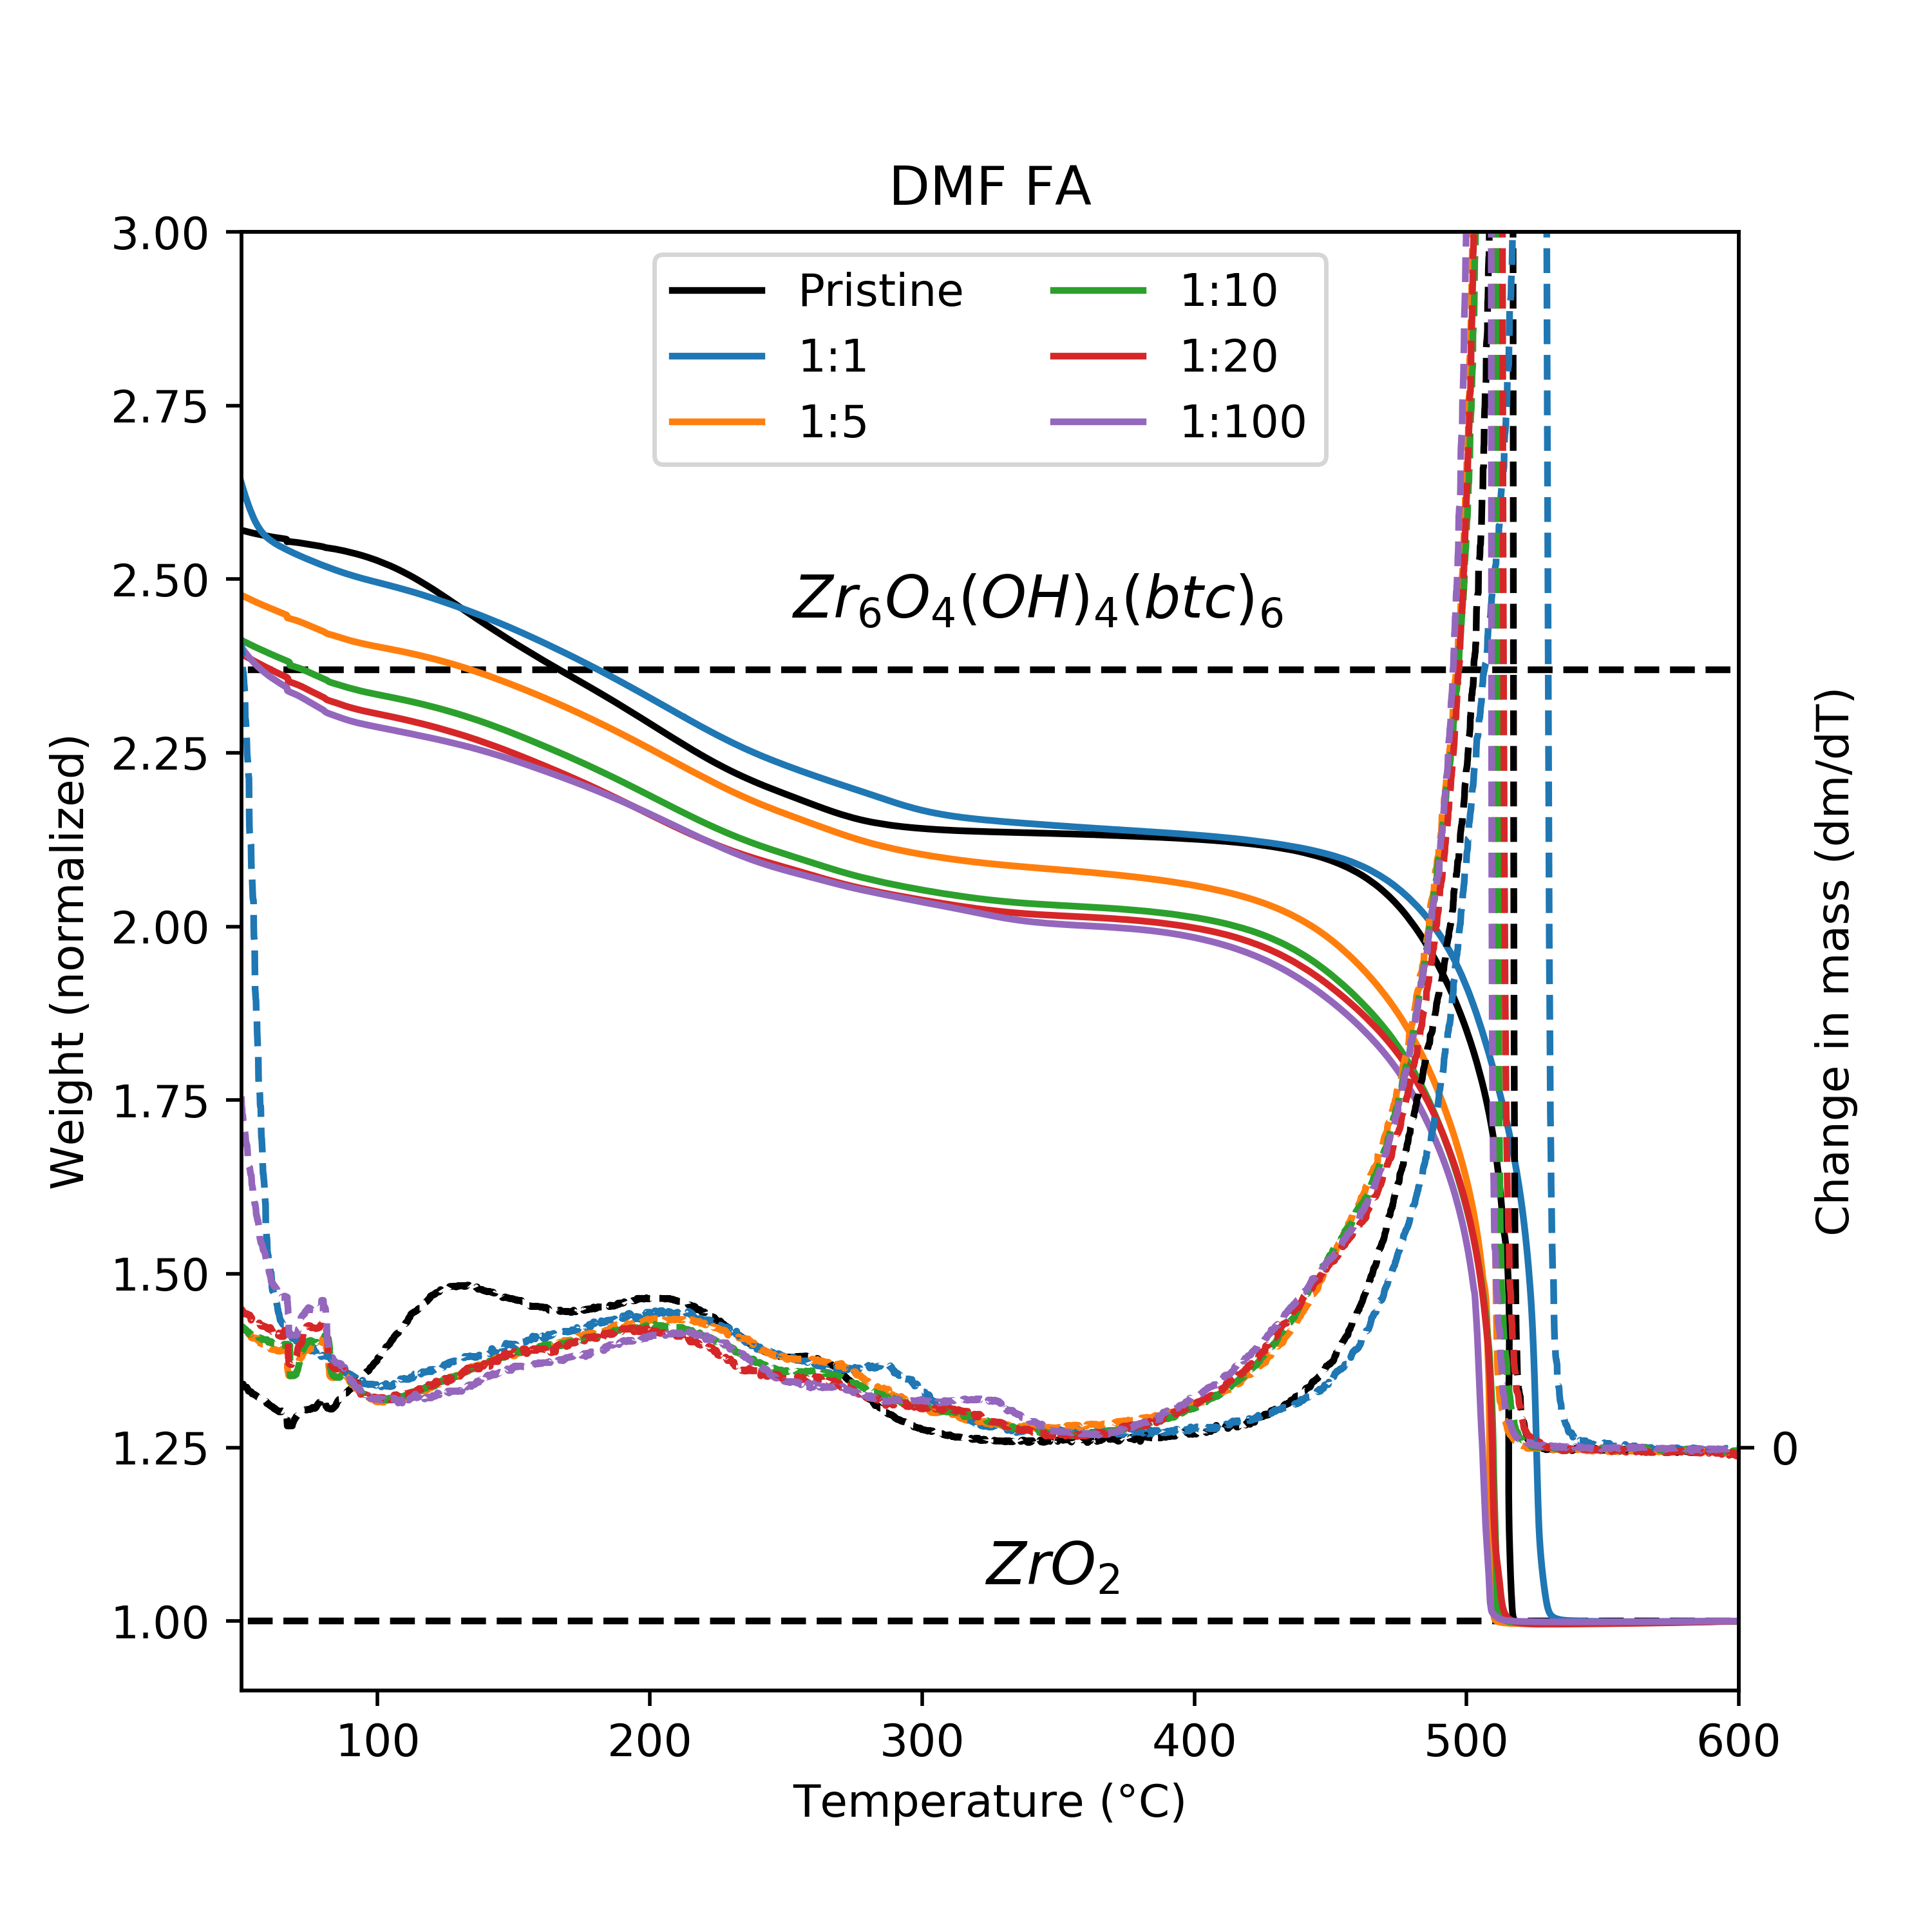
\includegraphics[width=\textwidth]{tga/DMF-FA}%
		\caption{}%
        \label{def:fgr:tga-dmf-fa}
    \end{subfigure}
    \begin{subfigure}{0.45\linewidth}
        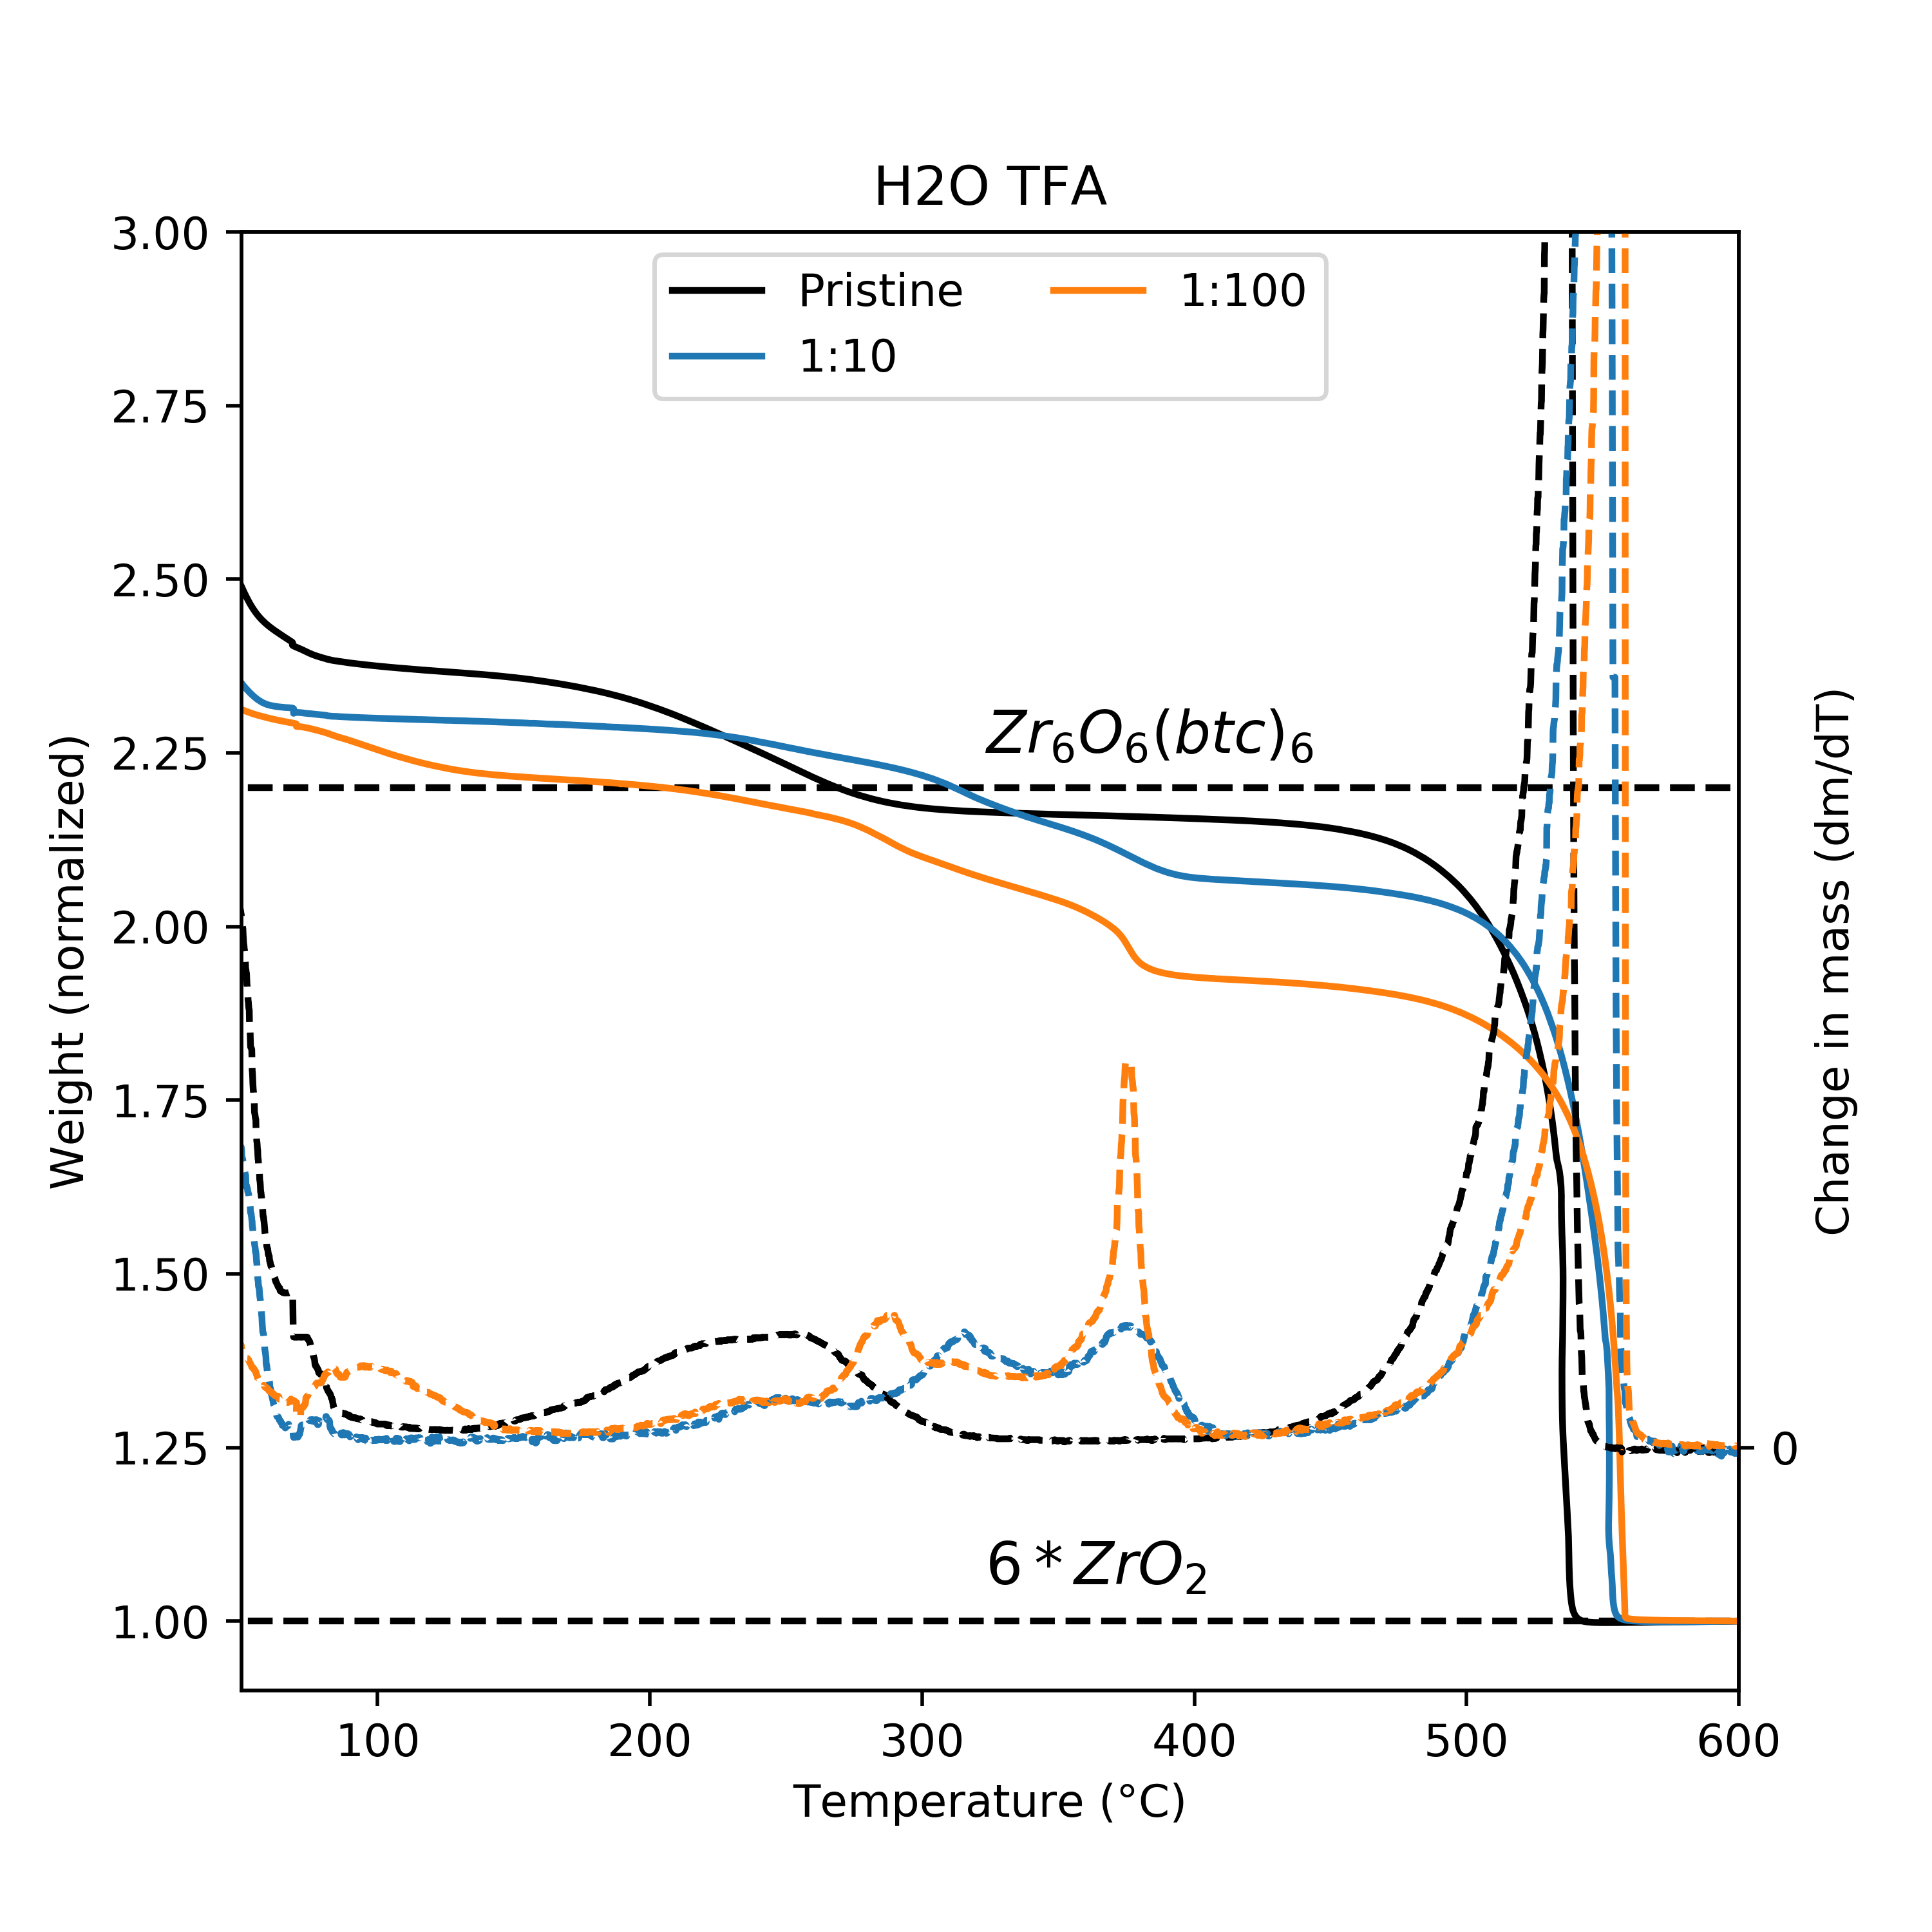
\includegraphics[width=\textwidth]{tga/H2O-TFA}%
		\caption{}%
        \label{def:fgr:tga-h2o-tfa}
    \end{subfigure}

    
    \begin{subfigure}{0.45\linewidth}
        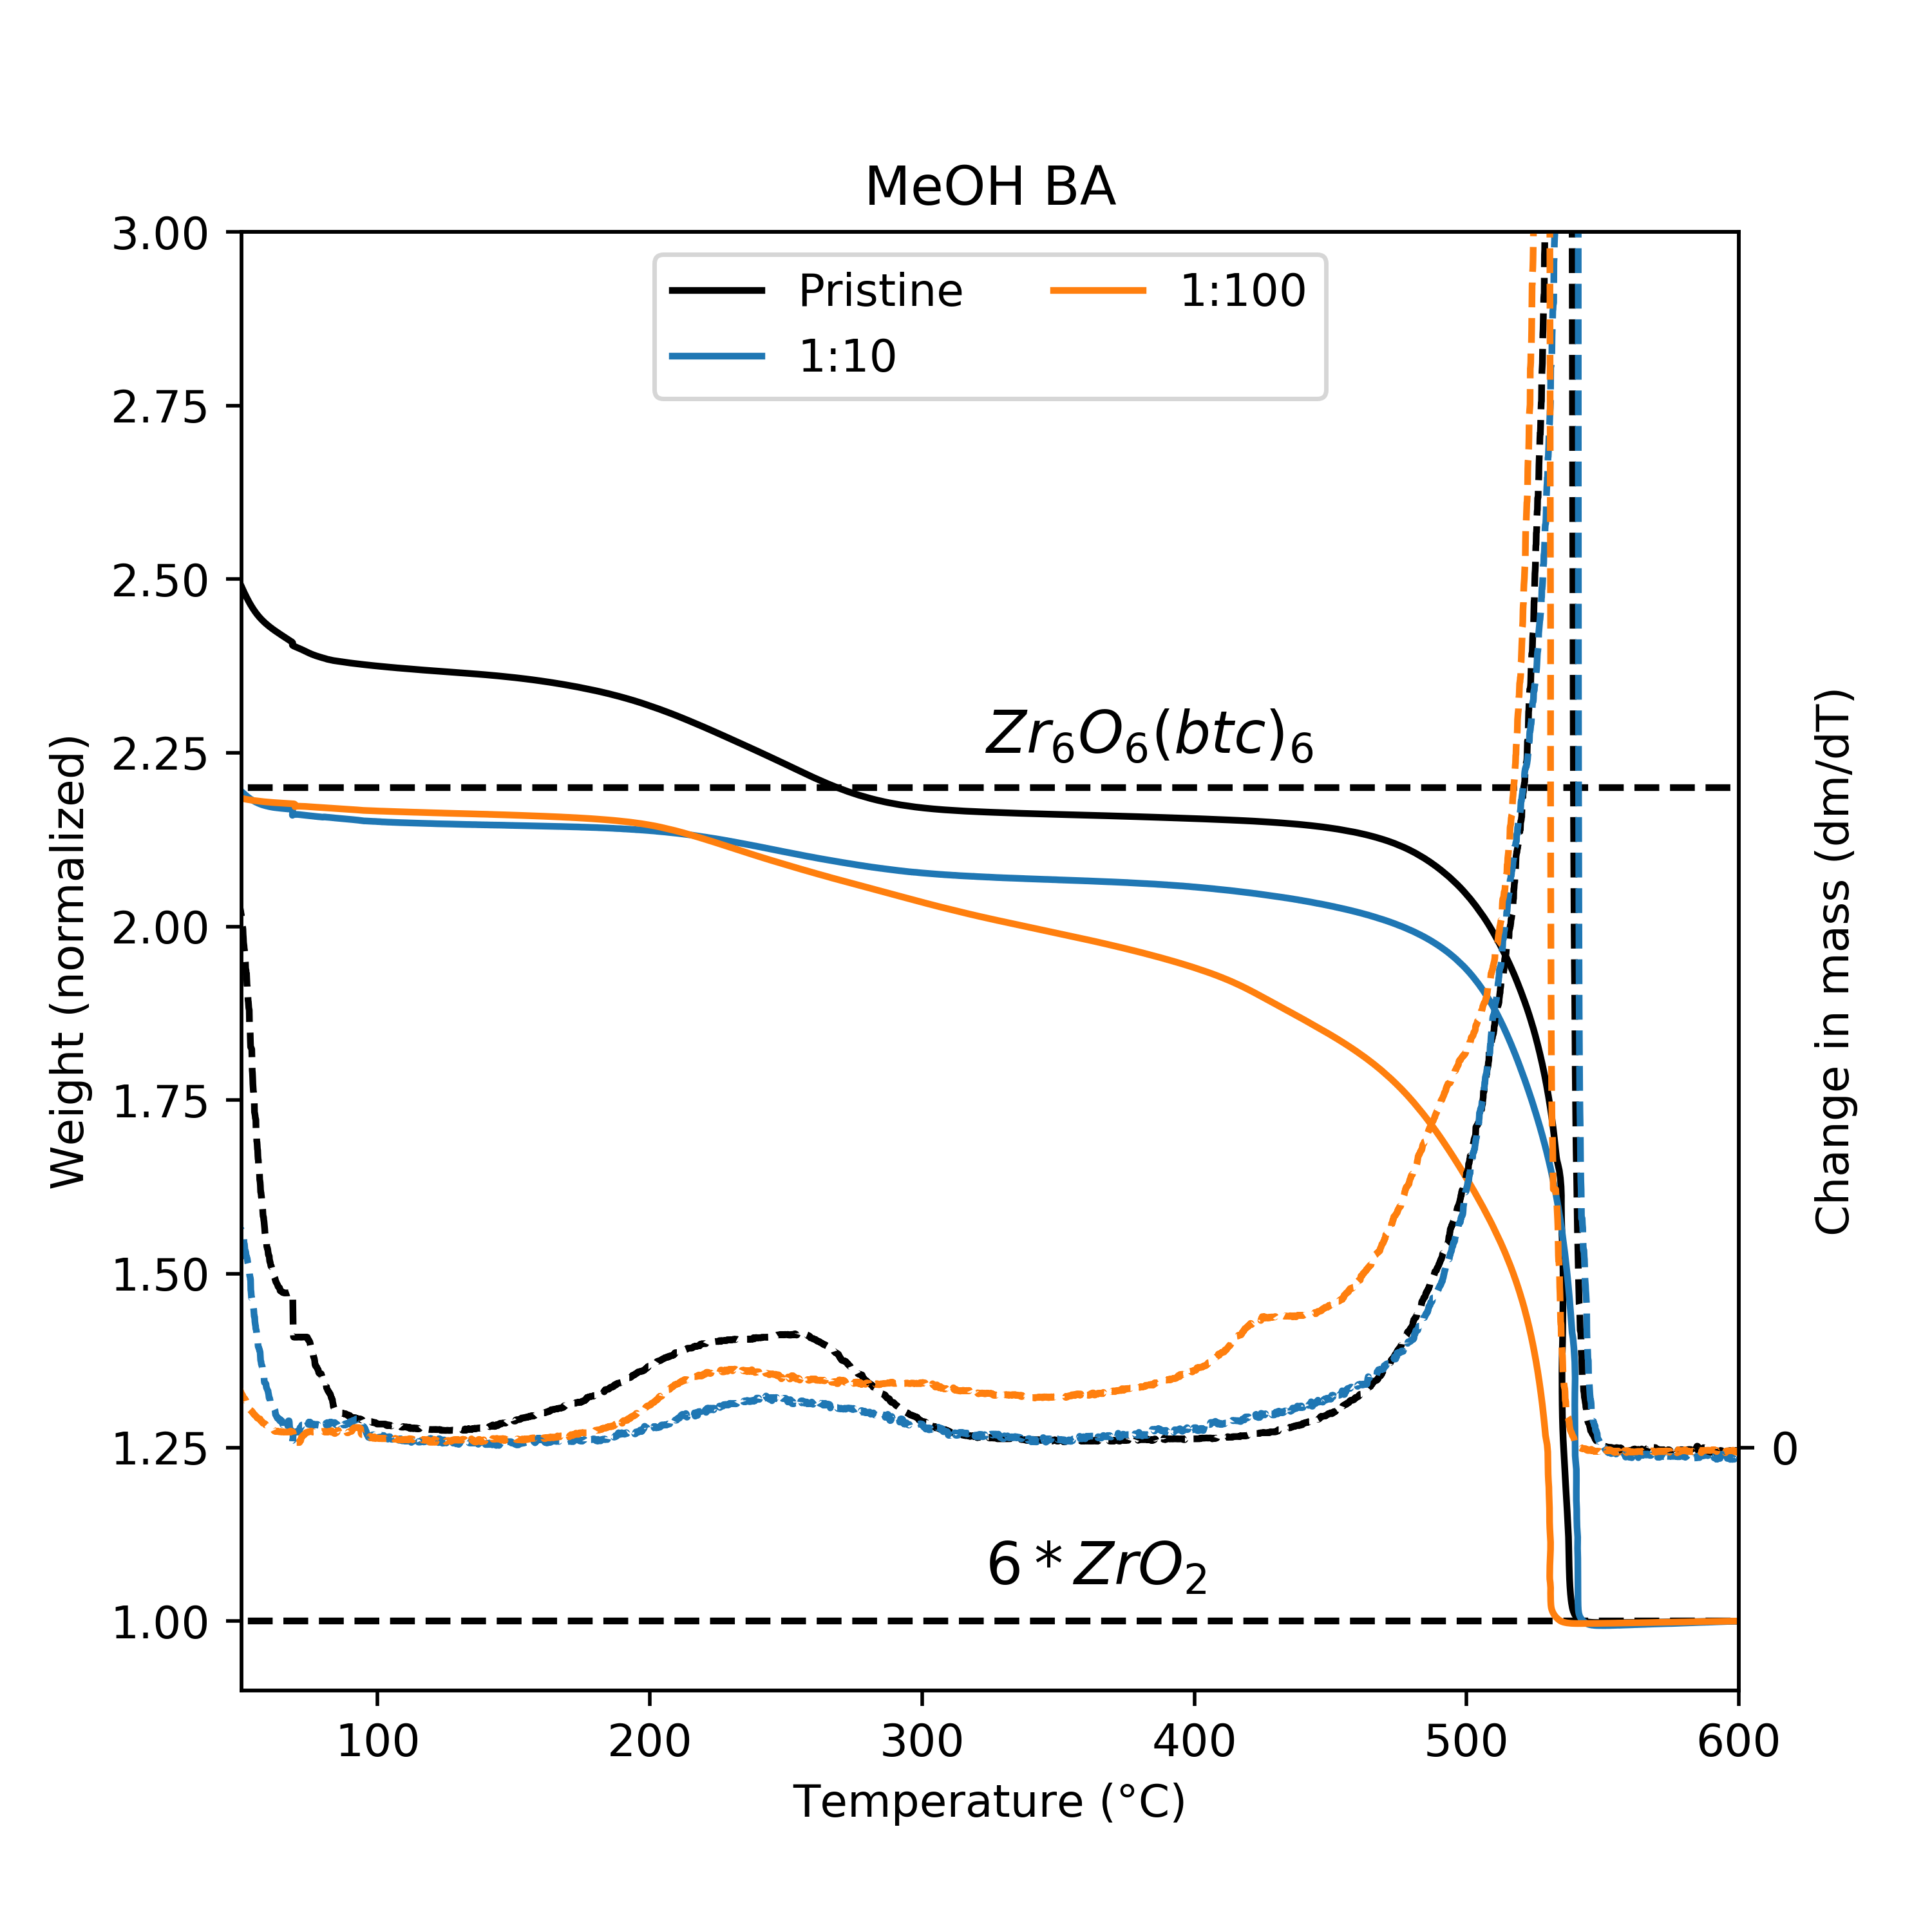
\includegraphics[width=\textwidth]{tga/MeOH-BA}%
		\caption{}%
        \label{def:fgr:tga-meoh-ba}
    \end{subfigure}
    \begin{subfigure}{0.45\linewidth}
        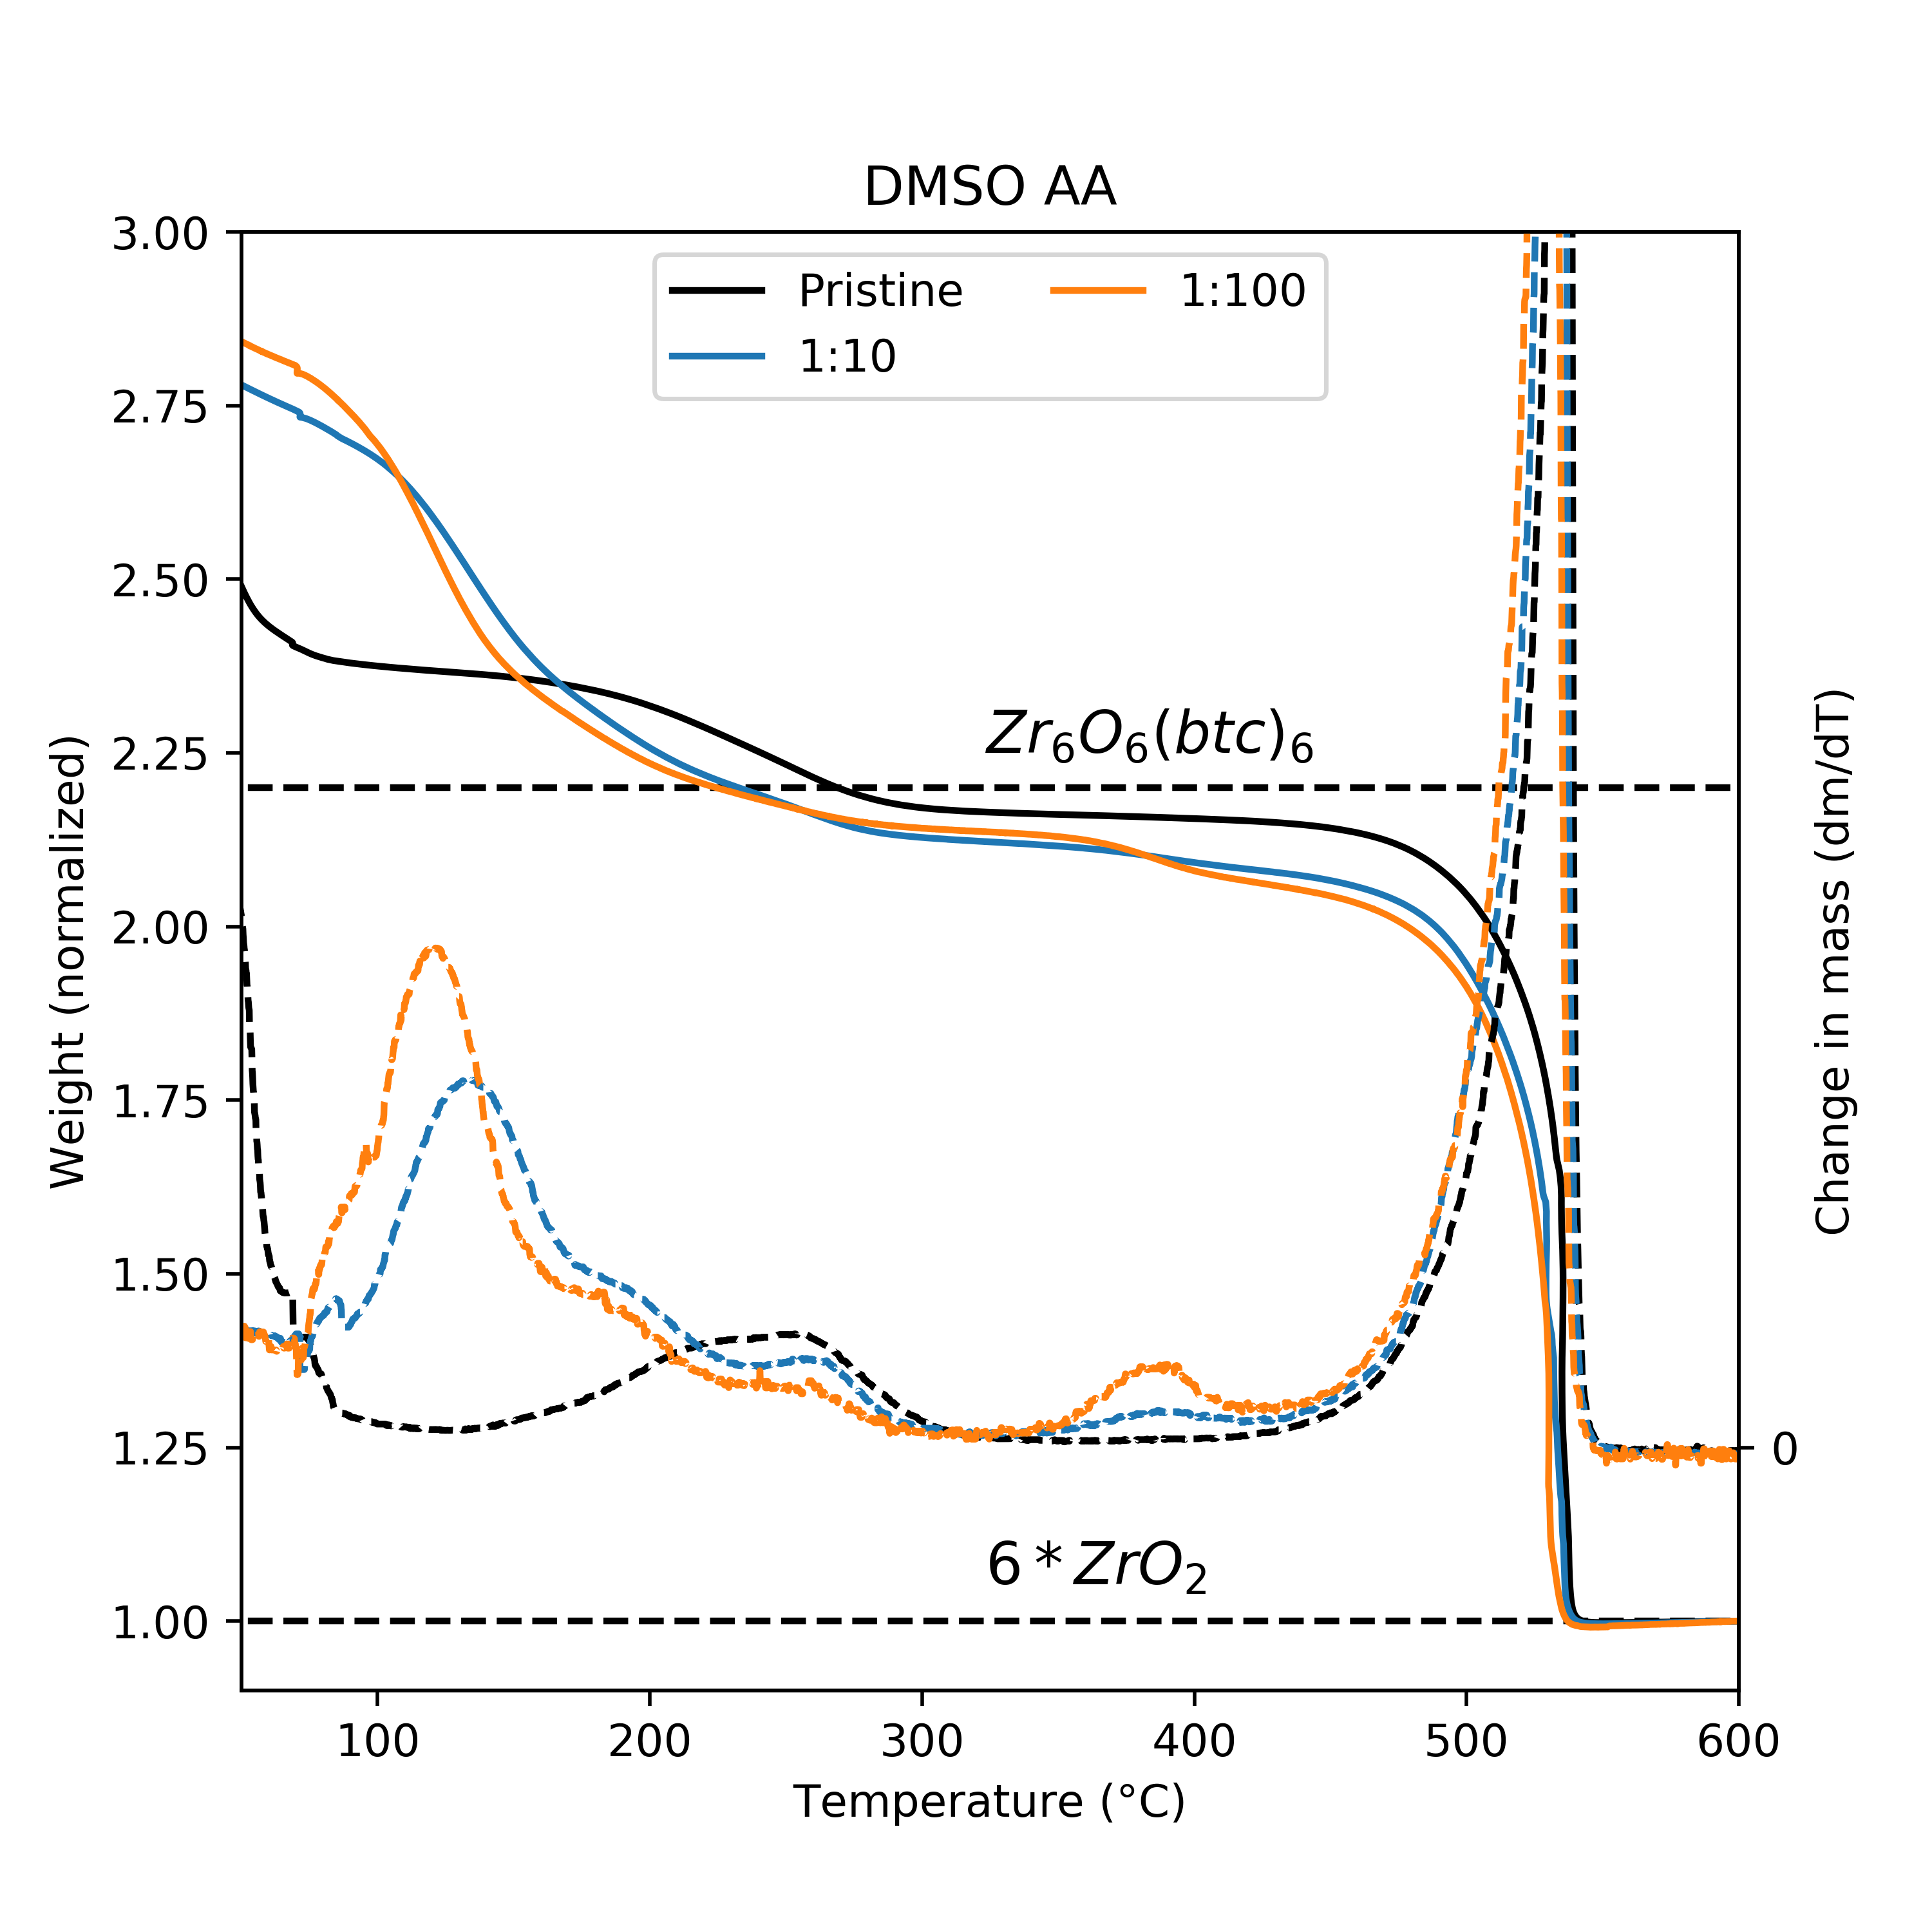
\includegraphics[width=\textwidth]{tga/DMSO-AA}%
		\caption{}%
        \label{def:fgr:tga-dmso-aa}
    \end{subfigure}

    \caption{A selection of the TGA curves as measured on the
    leached samples: (a) formic acid in DMF, (b) trifluoroacetic
    acid in water, (c) benzoic acid in methanol and (d) acetic acid
    in DMSO. The curve for the parent material is in black. 
    Dotted lines correspond to the secondary y axis as a 
    semilogarithm of the first derivative of mass loss with 
    respect to temperature.}%
    \label{def:fgr:tga-dataset}
\end{figure}

In leached samples where other acids were present,
it is likely that the original formate capping the defects 
has been replaced with an acid molecule from solution,
purely through kinetic means due to the large excess.
As evidenced in \autoref{def:fgr:tga-defects}, the mass 
loss corresponding to the formate is reduced, or no longer present. 
Acetic acid (\autoref{def:fgr:tga-dmso-aa}) leaves the 
structure at a higher temperature, as 
a new peak is present at \SI{390}{\degreeCelsius}.
Benzoic acid (\autoref{def:fgr:tga-meoh-ba}) introduces a progressive 
mass loss near the total decomposition temperature of \SI{550}{\degreeCelsius}.
As it is similar to the btc linker, its higher stability
is not surprising. Finally, the samples leached with 
TFA have a more complicated curve, with two or even 
three peaks in the derivative with respect to temperature.

The solvent used can be removed in all cases before 
\SI{200}{\degreeCelsius}. DMSO is the one with the highest
preponderence in the leached samples (\autoref{def:fgr:tga-dmso-aa}) 
and the most difficult to remove, likely due to its high boiling point.

The graphs in \autoref{def:fgr:tga-defects} summarize the 
trends in missing linker defects as calculated through 
the plateau at \SI{420}{\degreeCelsius}. Several clear trends can be 


\begin{figure}[htb]
    \centering

    \begin{subfigure}{0.45\linewidth}
        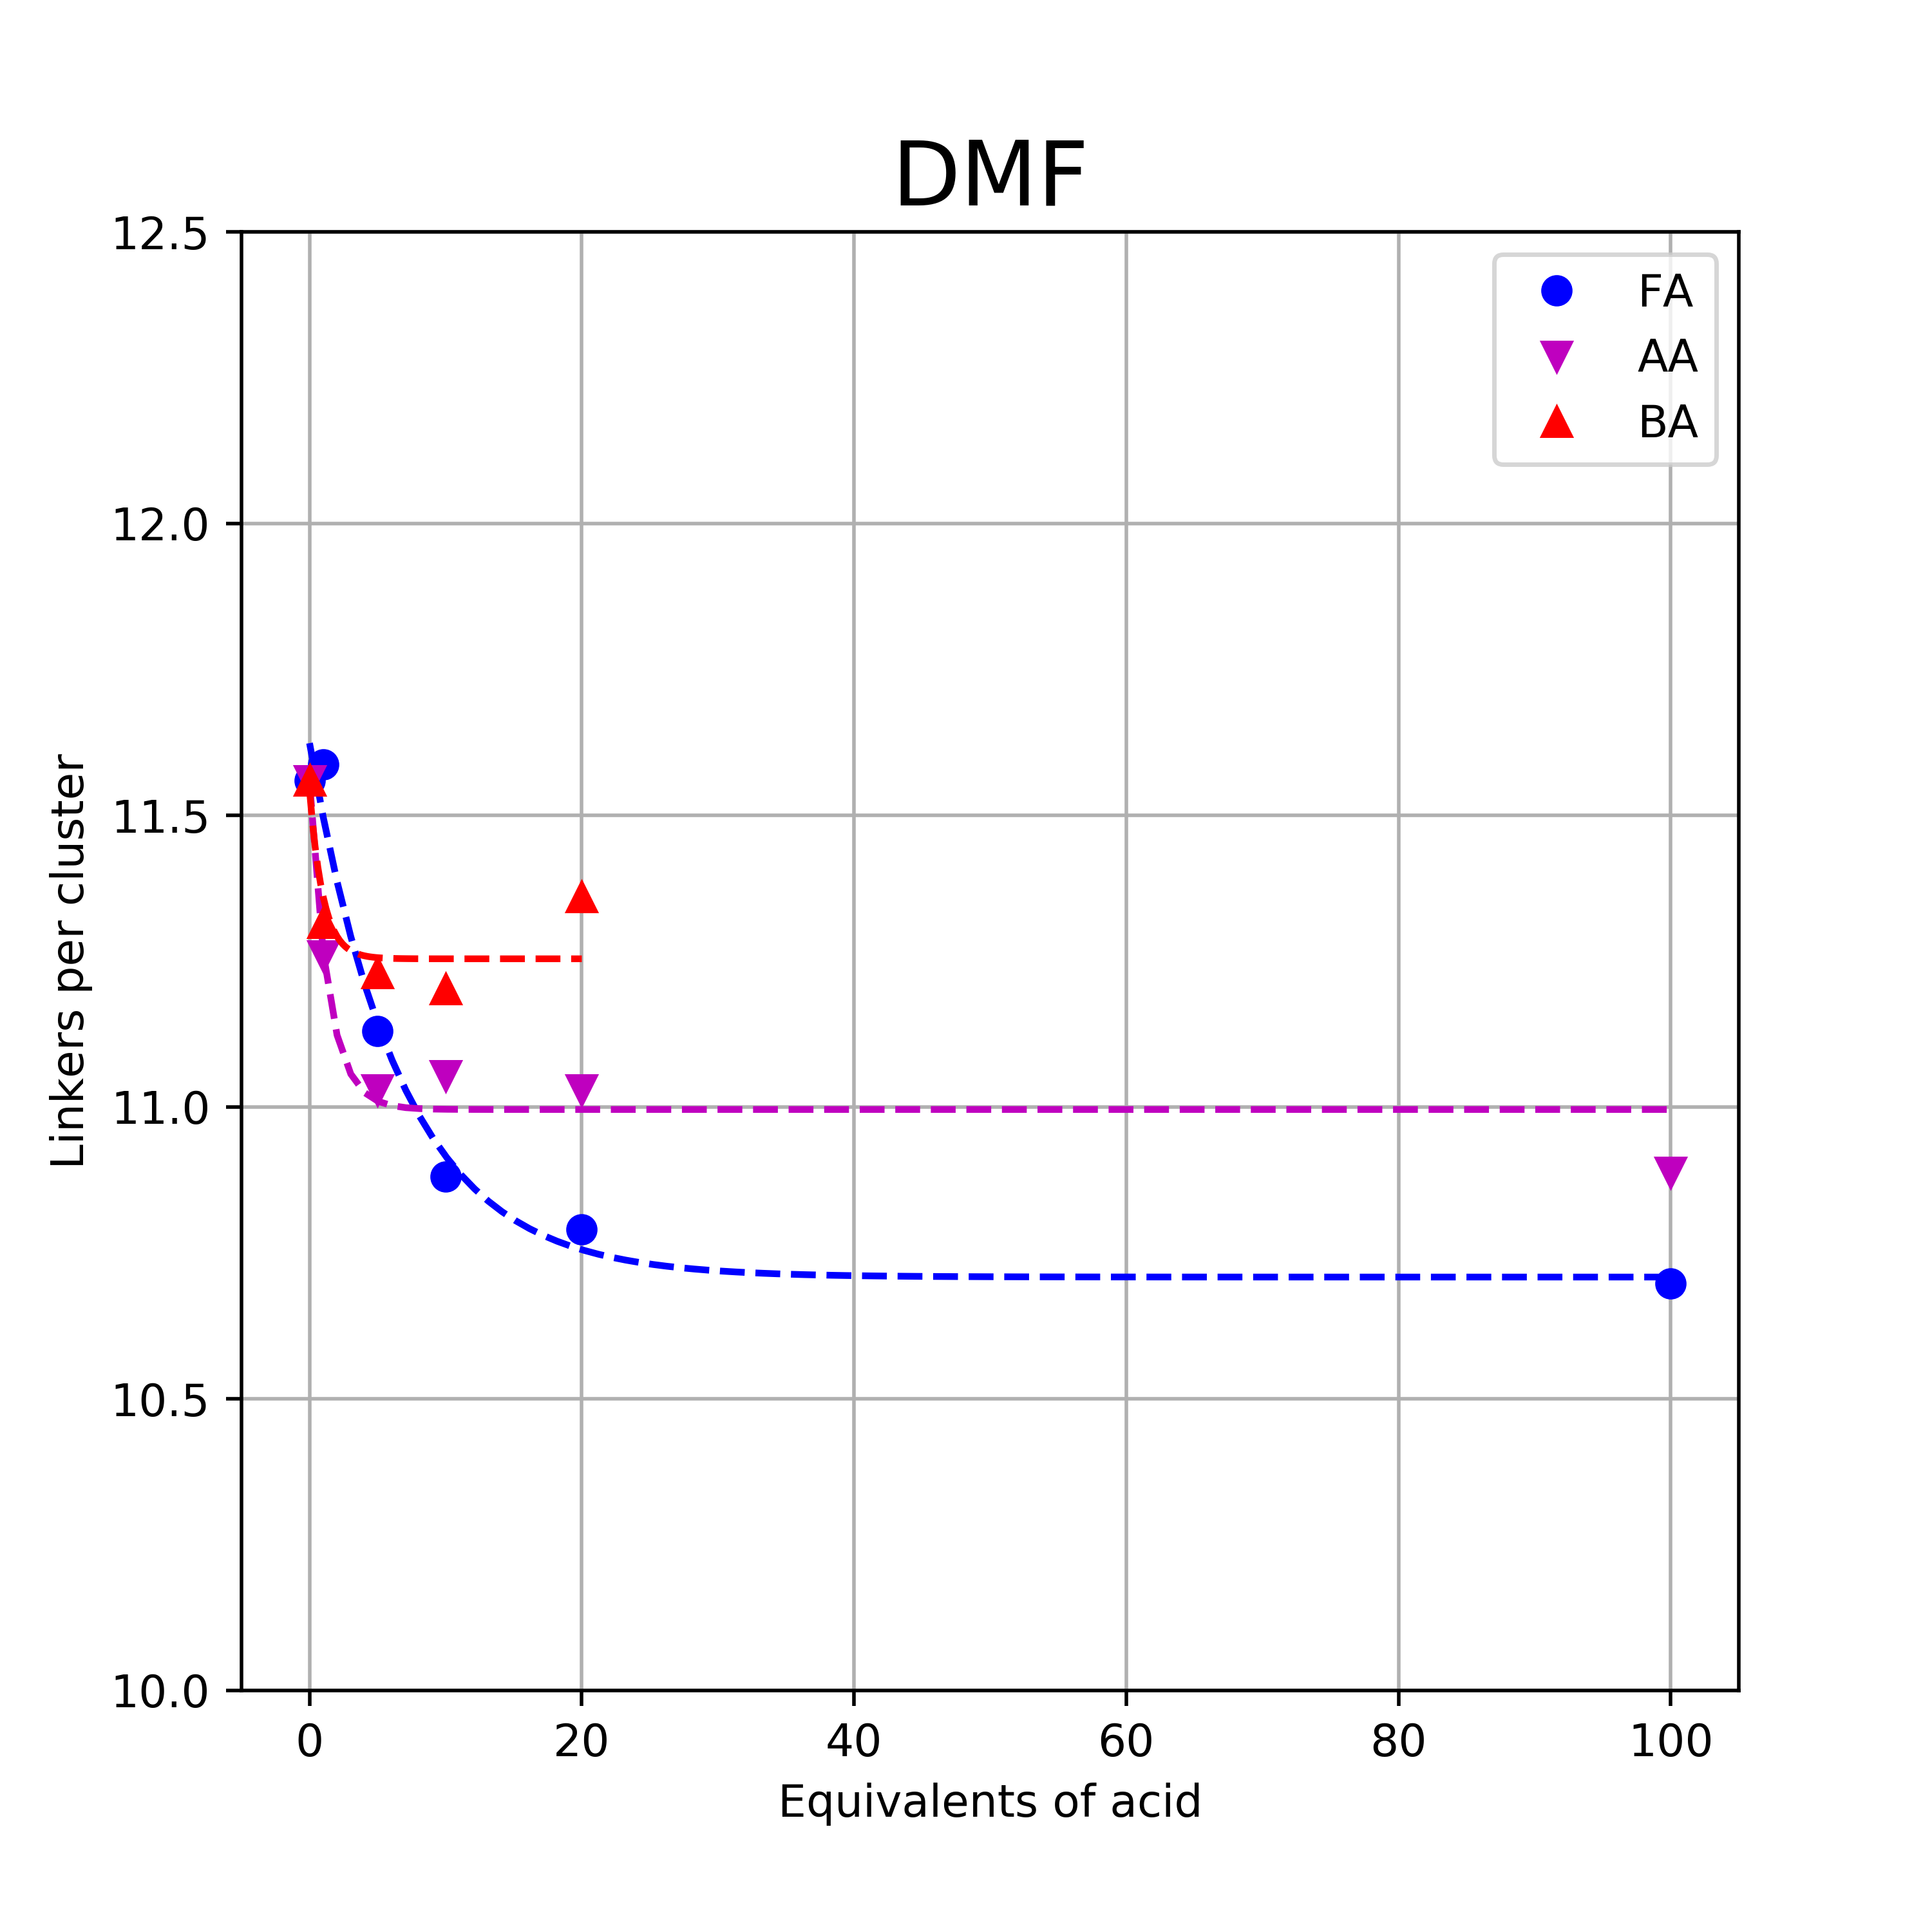
\includegraphics[width=\textwidth]{tga/DMF-def-overview}%
        \label{def:fgr:tga-dmf-linkers}
    \end{subfigure}
    \begin{subfigure}{0.45\linewidth}
        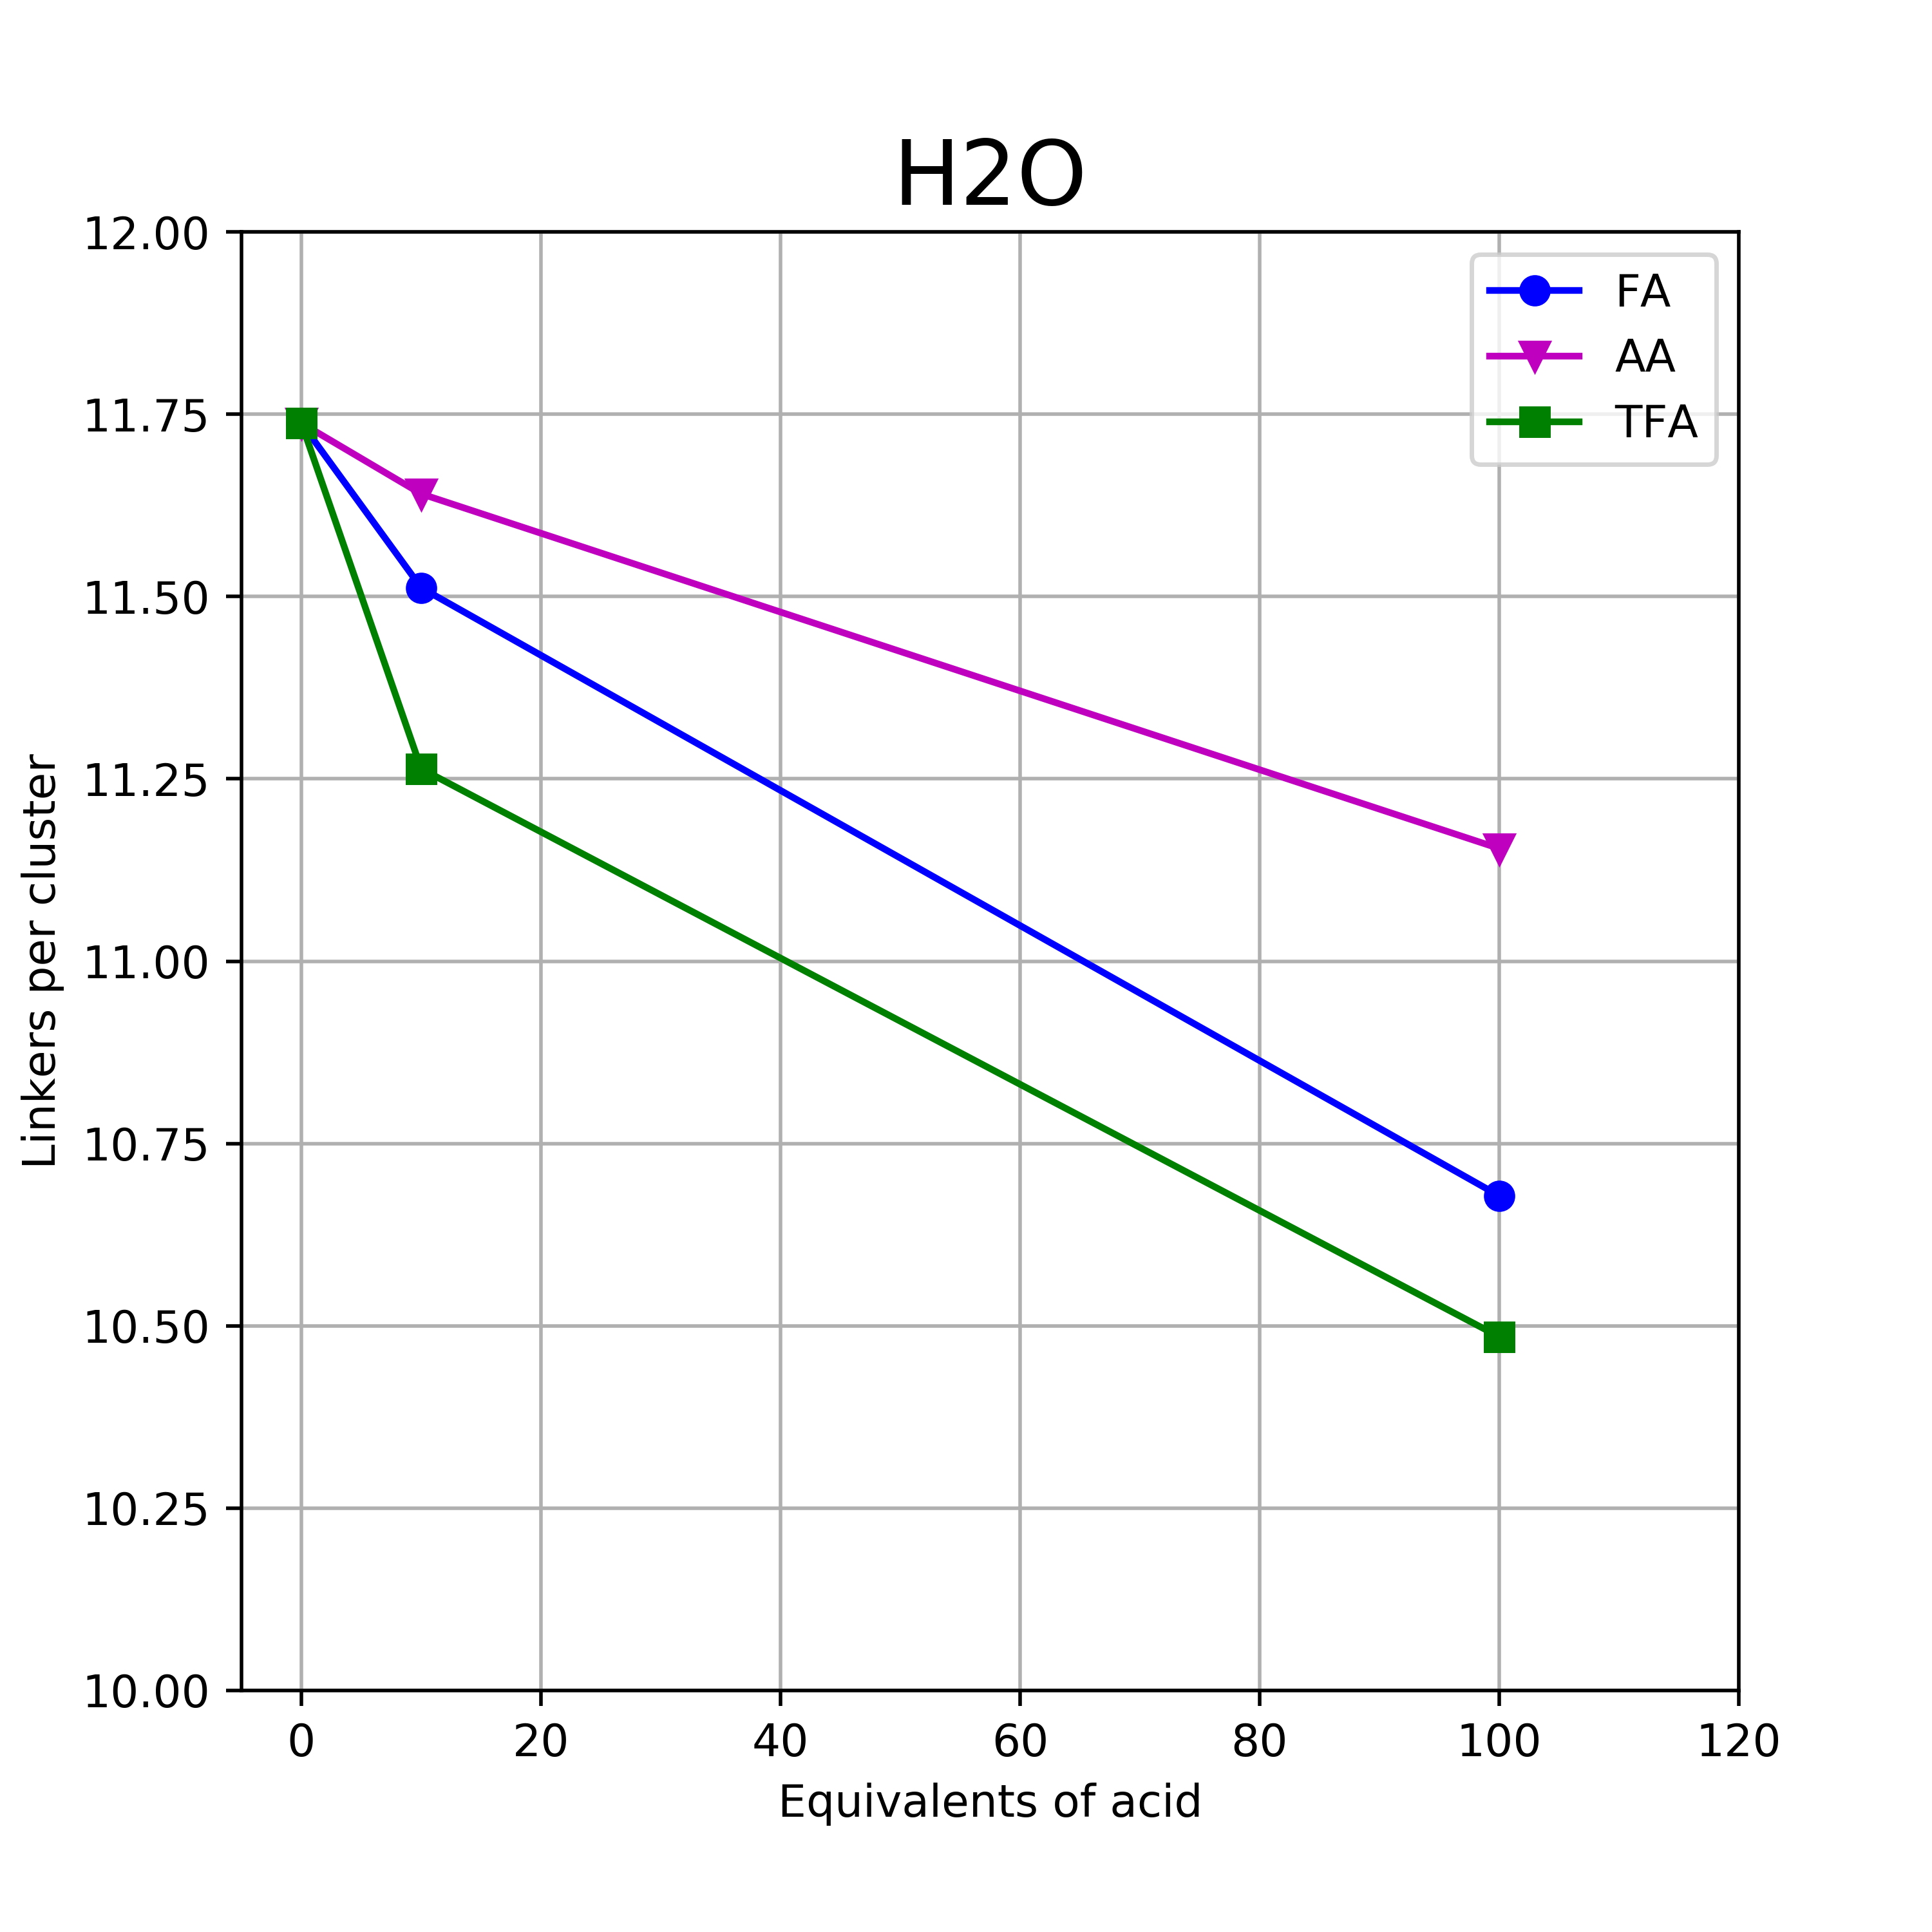
\includegraphics[width=\textwidth]{tga/H2O-def-overview}%
        \label{def:fgr:tga-h2o-linkers}
    \end{subfigure}

    
    \begin{subfigure}{0.45\linewidth}
        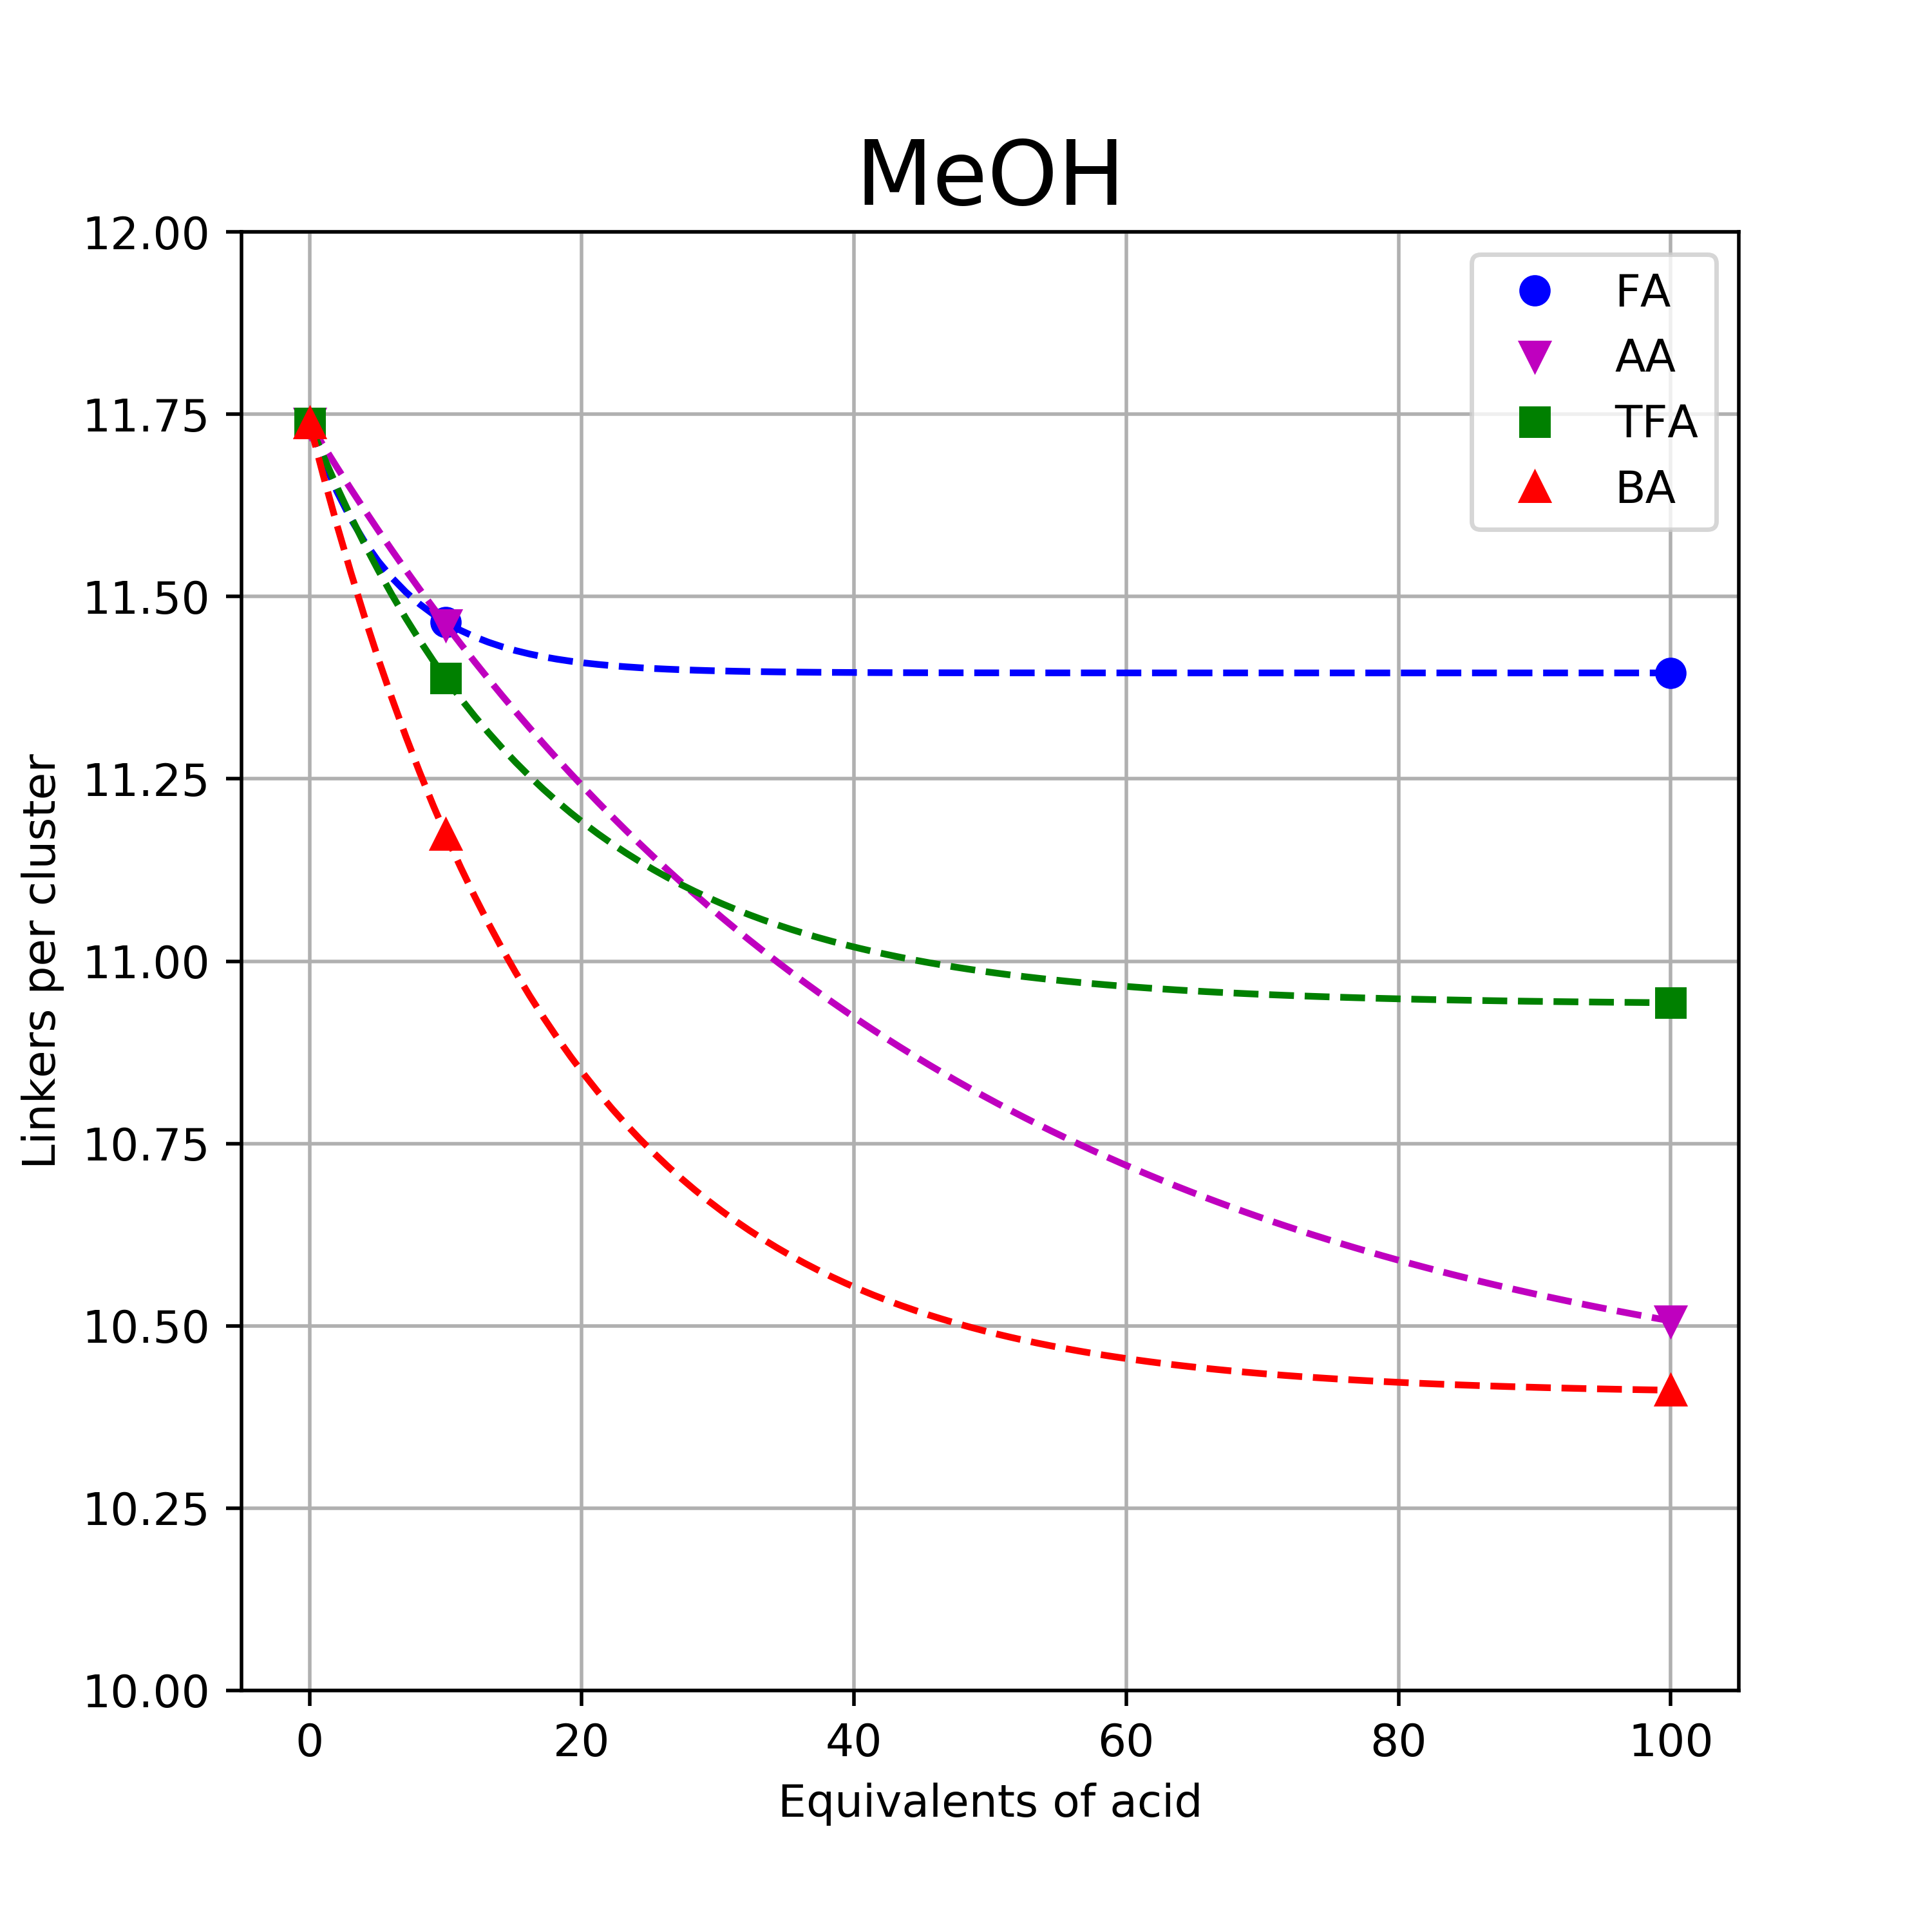
\includegraphics[width=\textwidth]{tga/MeOH-def-overview}%
        \label{def:fgr:tga-meoh-linkers}
    \end{subfigure}
    \begin{subfigure}{0.45\linewidth}
        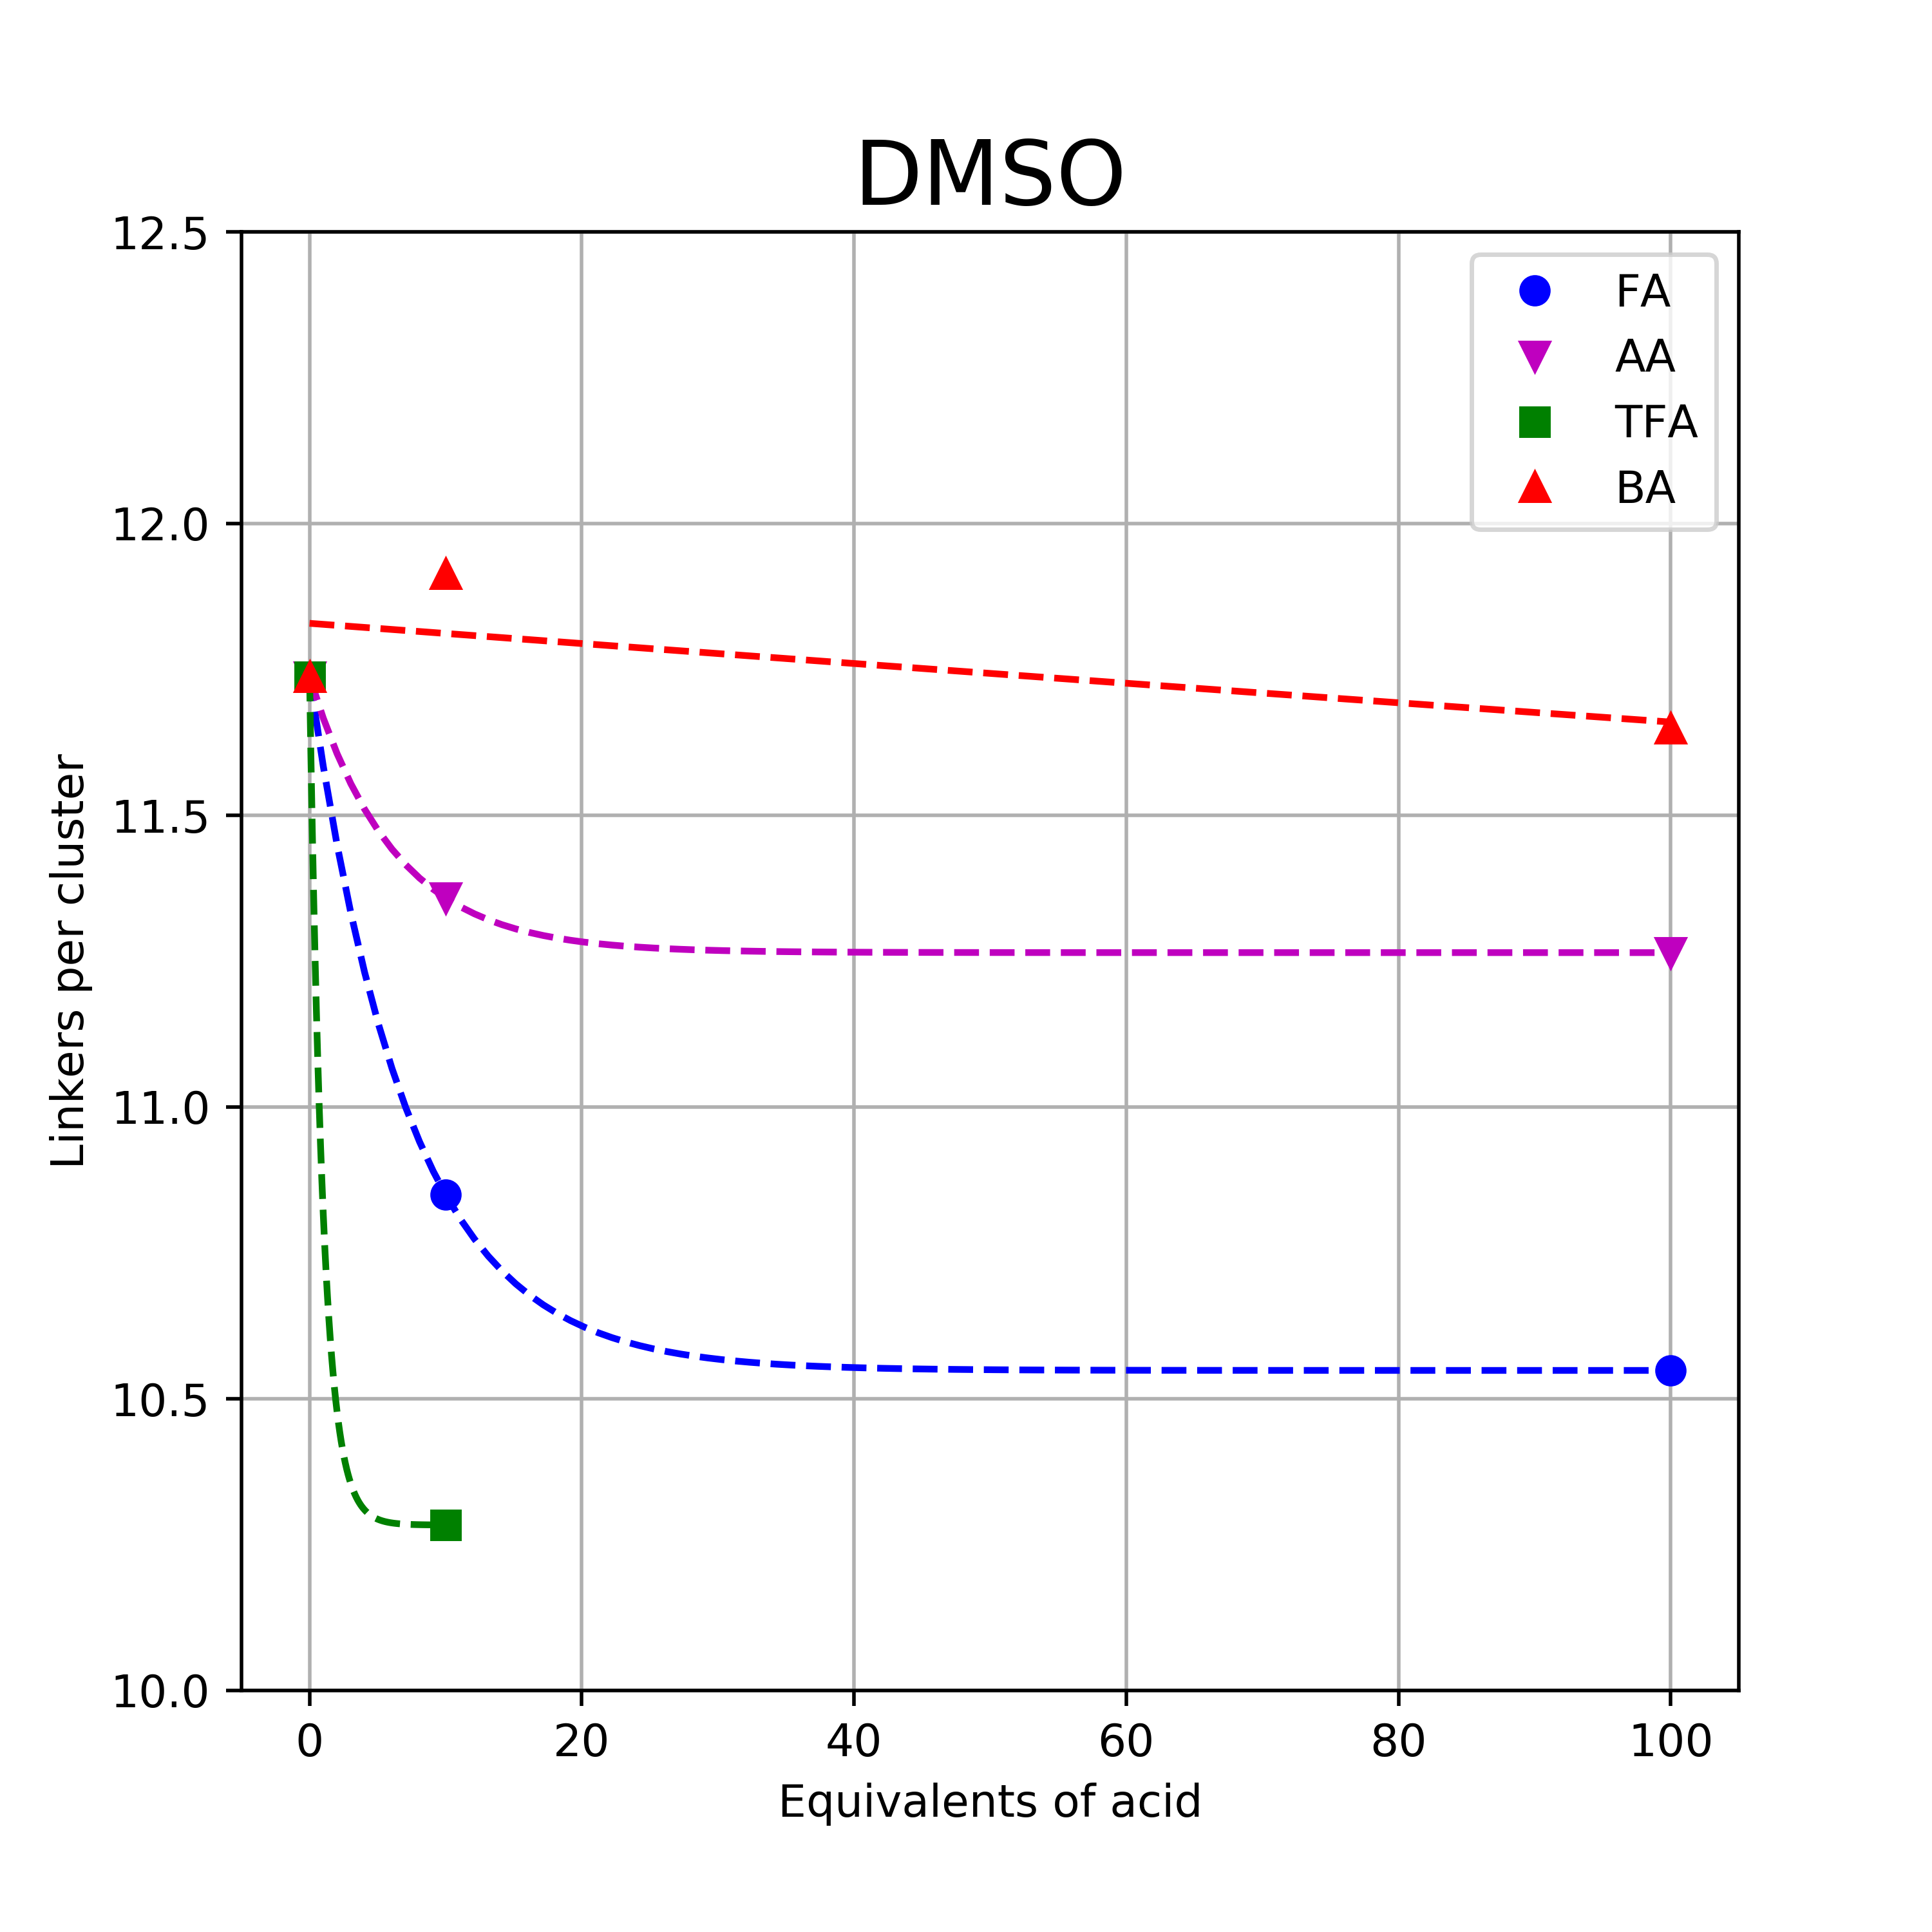
\includegraphics[width=\textwidth]{tga/DMSO-def-overview}%
        \label{def:fgr:tga-dmso-linkers}
    \end{subfigure}

    \caption{Calculated linker-to-node ratio from the TGA curve 
    normalized mass at \SI{420}{\degreeCelsius} for (a) DMF 
    (b) \ce{H2O}, (c) \ce{MeOH} and (d) DMSO leached samples.
    A ratio of 12 to 1 corresponds to a completely defect-free
    structure.}%
    \label{def:fgr:tga-defects}
    
\end{figure}


When DMF is used as a solvent, the resulting leached samples 
have a 

Since multiple concentrations of modulator were used only with 
DMF, inly a general trend is available.